\documentclass[12pt]{article}
\usepackage{geometry} % Pour passer au format A4
\geometry{hmargin=1cm, vmargin=1cm} % 

% Page et encodage
\usepackage[T1]{fontenc} % Use 8-bit encoding that has 256 glyphs
\usepackage[english,french]{babel} % Français et anglais
\usepackage[utf8]{inputenc} 

\usepackage{lmodern}
\setlength\parindent{0pt}

% Graphiques
\usepackage{graphicx,float,grffile}

% Maths et divers
\usepackage{amsmath,amsfonts,amssymb,amsthm,verbatim}
\usepackage{multicol,enumitem,url,eurosym,gensymb}

% Sections
\usepackage{sectsty} % Allows customizing section commands
\allsectionsfont{\centering \normalfont\scshape}

% Tête et pied de page

\usepackage{fancyhdr} 
\pagestyle{fancyplain} 

\fancyhead{} % No page header
\fancyfoot{}

\renewcommand{\headrulewidth}{0pt} % Remove header underlines
\renewcommand{\footrulewidth}{0pt} % Remove footer underlines

\newcommand{\horrule}[1]{\rule{\linewidth}{#1}} % Create horizontal rule command with 1 argument of height

%----------------------------------------------------------------------------------------
%	Début du document
%----------------------------------------------------------------------------------------

\begin{document}

%----------------------------------------------------------------------------------------
% RE-DEFINITION
%----------------------------------------------------------------------------------------
% MATHS
%-----------

\newtheorem{Definition}{Définition}
\newtheorem{Theorem}{Théorème}
\newtheorem{Proposition}{Propriété}

% MATHS
%-----------
\renewcommand{\labelitemi}{$\bullet$}
\renewcommand{\labelitemii}{$\circ$}
%----------------------------------------------------------------------------------------
%	Titre
%----------------------------------------------------------------------------------------

\setlength{\columnseprule}{1pt}

\section*{ie 2 - Théorème de Pythagore}
\begin{center}
  \textit{Théophraste- La plus coûteuse des dépenses, c’est la perte de temps.}
\end{center}
\horrule{2px}

\begin{multicols}{2}
  \begin{itemize}
  \item S'organiser : Avoir sa calculatrice.
  \item Communiquer : Soin général.
  \item Connaissance : Théorème de Pythagore.
  \item Raisonner : Rédiger la démarche.
  \item Calculer : Trouver le bon résultat.
  \end{itemize}
\end{multicols}


\subsection*{Restituer}

\textbf{Restituer} le théorème de Pythagore.

\subsection*{Ex1 - S'entraîner}


\begin{multicols}{2}
  \begin{enumerate}
  \item[1.] Soit $OCB$ un triangle rectangle en $B$ tel que :\\
    $OB=4,8cm \text{ et }CO=8cm$.\\
    Calculer la longueur $CB$.
    \columnbreak
  \item[2.] Soit $BQZ$ un triangle rectangle en $B$ tel que : \\
    $QB=12cm \text{ et } ZB=16cm$.\\
    Calculer la longueur $ZQ$.
  \end{enumerate}
\end{multicols}


\begin{multicols}{2}
  \begin{enumerate}
  \item[3.] Soit $WUN$ un triangle rectangle en $N$ tel que :\\
    $WN=10cm \text{ et }UW=14,5cm$.\\
    Calculer la longueur $UN$.
    \columnbreak
  \item[4.] Soit $FER$ un triangle rectangle en $E$ tel que :\\
    $FE=4cm \text{ et }RE=3cm$.\\
    Calculer la longueur $FR$.
  \end{enumerate}
\end{multicols}


\begin{multicols}{2}
  \begin{enumerate}
  \item[5.] Soit $UAB$ un triangle rectangle en $B$ tel que :\\
    $AU=8cm \text{ et }AB=6,4cm$.\\
    Calculer la longueur $UB$.
    \columnbreak
  \item[6.] Soit $JOD$ un triangle rectangle en $J$ tel que :\\
    $OJ=8,4cm \text{ et }DJ=6,3cm$.\\
    Calculer la longueur $OD$.
  \end{enumerate}
\end{multicols}

\subsection*{Ex2 - Situation de problème}

Peut-on recouvrir entièrement une table rectangulaire de 120 cm de long et de 80 cm de large par une nappe ronde de 130 cm de diamètre ?

\begin{enumerate}
\item[1.] \textbf{Représenter} la situation. Faire un schéma de la situation, \textit{avec les longueurs, la règle, ...}
\item[2.] Justifier pourquoi on peut utiliser le théorème de Pythagore pour résoudre ce problème. \textbf{Modéliser}. 
\item[3.] Résoudre la situation. \textbf{Raisonner}
\end{enumerate}

\begin{multicols}{2}
  \begin{figure}[H]
    \centering
    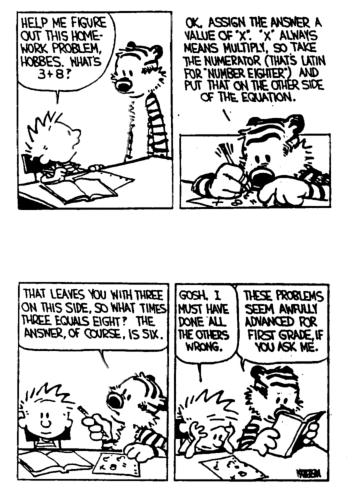
\includegraphics[width=0.6 \linewidth]{4x1-pythagore/sources/cah.jpg}
  \end{figure}

  \subsection*{Bonus - Traduire}

\end{multicols}

\newpage

\section*{ie 2 - Théorème de Pythagore}
\begin{center}
  \textit{Théophraste- La plus coûteuse des dépenses, c’est la perte de temps.}
\end{center}
\horrule{2px}

\begin{multicols}{2}
  \begin{itemize}
  \item S'organiser : Avoir sa calculatrice.
  \item Communiquer : Soin général.
  \item Connaissance : Théorème de Pythagore.
  \item Raisonner : Rédiger la démarche.
  \item Calculer : Trouver le bon résultat.
  \end{itemize}
\end{multicols}


\subsection*{Restituer}

\textbf{Restituer} le théorème de Pythagore.

\subsection*{Ex1 - S'entraîner}

\begin{multicols}{2}
    \begin{enumerate}
    \item[1.] Soit $YUW$ un triangle rectangle en $Y$ tel que :\\
      $WU= 3,7cm \text{ et }WY= 3,5cm$.\\
      Calculer la longueur $UY$.
      \columnbreak
    \item[2.] Soit $QSK$ un triangle rectangle en $Q$ tel que :\\
      $KQ= 9cm \text{ et }SQ= 4,8cm$.\\
      Calculer la longueur $KS$.
    \end{enumerate}
  \end{multicols}


  \begin{multicols}{2}
    \begin{enumerate}
    \item[3.] Soit $EHK$ un triangle rectangle en $K$ tel que :\\
      $EK= 3,6cm \text{ et }HK= 1,5cm$.\\
      Calculer la longueur $EH$.
      \columnbreak
    \item[4.] Soit $XSM$ un triangle rectangle en $S$ tel que :\\
      $MS= 11,4cm \text{ et }XM= 19cm$.\\
      Calculer la longueur $XS$.
    \end{enumerate}
  \end{multicols}



  \begin{multicols}{2}
    \begin{enumerate}
    \item[5.] Soit $LKT$ un triangle rectangle en $K$ tel que :\\
      $TK= 10,4cm \text{ et }LK= 7,8cm$.\\
      Calculer la longueur $TL$.
      \columnbreak
    \item[6.] Soit $VLR$ un triangle rectangle en $V$ tel que :\\
      $RV= 3,5cm \text{ et }LR= 9,1cm$.\\
      Calculer la longueur $LV$.
    \end{enumerate}
  \end{multicols}

\subsection*{Ex2 - Situation de problème}

Peut-on recouvrir entièrement une table rectangulaire de 120 cm de long et de 80 cm de large par une nappe ronde de 130 cm de diamètre ?

\begin{enumerate}
\item[1.] \textbf{Représenter} la situation. Faire un schéma de la situation, \textit{avec les longueurs, la règle, ...}
\item[2.] Justifier pourquoi on peut utiliser le théorème de Pythagore pour résoudre ce problème. \textbf{Modéliser}. 
\item[3.] Résoudre la situation. \textbf{Raisonner}
\end{enumerate}

\begin{multicols}{2}
  \begin{figure}[H]
    \centering
    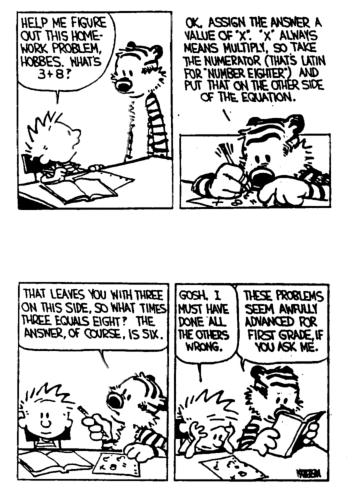
\includegraphics[width=0.6 \linewidth]{4x1-pythagore/sources/cah.jpg}
  \end{figure}

  \subsection*{Bonus - Traduire}

\end{multicols}

\end{document}
